\documentclass[letterpaper,12pt]{article}
\usepackage{tabularx} % extra features for tabular environment
\usepackage{amsmath}  % improve math presentation
\usepackage{float}
\usepackage{pdfpages}

\usepackage{graphicx} % takes care of graphic including machinery
\graphicspath{ {./figures/} }
\usepackage[margin=1in,letterpaper]{geometry} % decreases margins
\usepackage{cite} % takes care of citations
\usepackage[final]{hyperref} % adds hyper links inside the generated pdf file
\hypersetup{
	colorlinks=true,       % false: boxed links; true: colored links
	linkcolor=blue,        % color of internal links
	citecolor=blue,        % color of links to bibliography
	filecolor=magenta,     % color of file links
	urlcolor =blue         
}

%



\begin{document}

\title{EE213 Term Project \protect\\Pre-Design Report}
\author{Ahmet Akman 2442366}
\date{\today}
\maketitle
\newpage

\tableofcontents
\newpage

%\begin{abstract}
%abstract
%\end{abstract}

\section{Introduction and Project Objective}
In this document, the design aprroaches proposed for given term project of EE213. The term-project requirements can be basically summarized that, students are expected to design an experiment to measure the distance of a light source. It is given that the component "LDR (Light Dependent Resistor)" will be used as the sensor element. Also the basic passive components, Op-Amps and laboratory equipments are in the scope of use. The physical appearence of a photoresistor is given in the Figure 1. 
%%%%%%%%%%%%%%%%%%%%%Figure 1 LDR photo
As students, we are expected to prepare a proper experiment procedure including Pre-Lab work and testing phases. 
There are two measurement solutions to be proposed. The first one is constructed on the basic working principle of the photoresistor and properties of constant light sources. The second one is based on modified version of the Time of Flight solution which widely used in industrial distance measurement devices. Both proposals share the same objective of to be able to characterize light dependent resistor. Also the preliminary measurements and experiment results for the both approach is reported.


\section{Proposal 1}
In this section the first proposal is described.
\subsection{Linear Approach}
In this approach, the linear behavior of the LDR component against light intensity is aimed to be used. The setup simply includes a light source , an LDR and a multimeter connected to that LDR. The circuit schematic is given in the Figure 2.
%%%%%%%%%%%%%%%%%%%%%%%% FİGURE 2 circuit schematic
\subsubsection{Light Intensity and Distance Relation}
From the fundamentals of physics it is stated that the the light intensity caused by a single light source drops by inverse square of its distance. This is also illustrated in Figure 3.
%%%%%%%%%%%%%%%%%%%%%%% Figure 3 light intensity drops
This relation also mathematically modelled by the equation:
\[light intensity  = \frac{1}{distance}\]
\subsubsection{The LDR Component}
The Light Dependent Resistor(frequently abbrevieted as LDR), is a semiconductor component so that its  resistance changes when the illumination on its surface change. The resistance curve of an LDR is given in the Figure 4.
%%%%%%%%%%%%%%%%%%%%%%%%%%Figure 4 curve resistance
Although it seems this linear curve makes process pretty straightforward, real life conditions  (which we can not omit the daylight and ambient light).s
\subsection{Calibration Proccess}
\subsection{Distance Measurement Calculations}
\subsection{Preliminary Results}

\section{Proposal 2}
\subsection{Time of Flight Approach}
\subsection{Distance Measurement Calculations}
\subsection{Preliminary Results}

\section{Conclusion}



%++++++++++++++++++++++++++++++++++++++++
% References section will be created automatically 
% with inclusion of "thebibliography" environment
% as it shown below. See text starting with line
% \begin{thebibliography}{99}
% Note: with this approach it is YOUR responsibility to put them in order
% of appearance.

%\begin{thebibliography}{99}

%https://tr.overleaf.com/latex/templates/sample-lab-report-for-u-of-r-phys-349/pgsyqngcyjxk

%\end{thebibliography}


\end{document}


\begin{table}[H]
	\begin{center}
		\caption{Resistance reading by color code convention.}
		\vspace{2mm}
		\begin{tabular}{||c | c | c||} 
		 \hline
		 Color Order & Value & Tolerance \\ [0.5ex] 
		 \hline\hline
		 Brown / Black / Red / Gold & 1k\( \Omega \) & \( \% \) 5  \\ 
		 \hline
		 Yellow / Violet / Red / Gold & 4.7k\( \Omega \) & \( \% \) 5   \\
		 \hline
		 Brown / Grey / Orange / Gold & 18k\( \Omega \) & \( \% \) 5  \\ [1ex] 
		 \hline
		\end{tabular}
	\end{center}
	\end{table}

	\begin{figure}[H]
 		\centering
		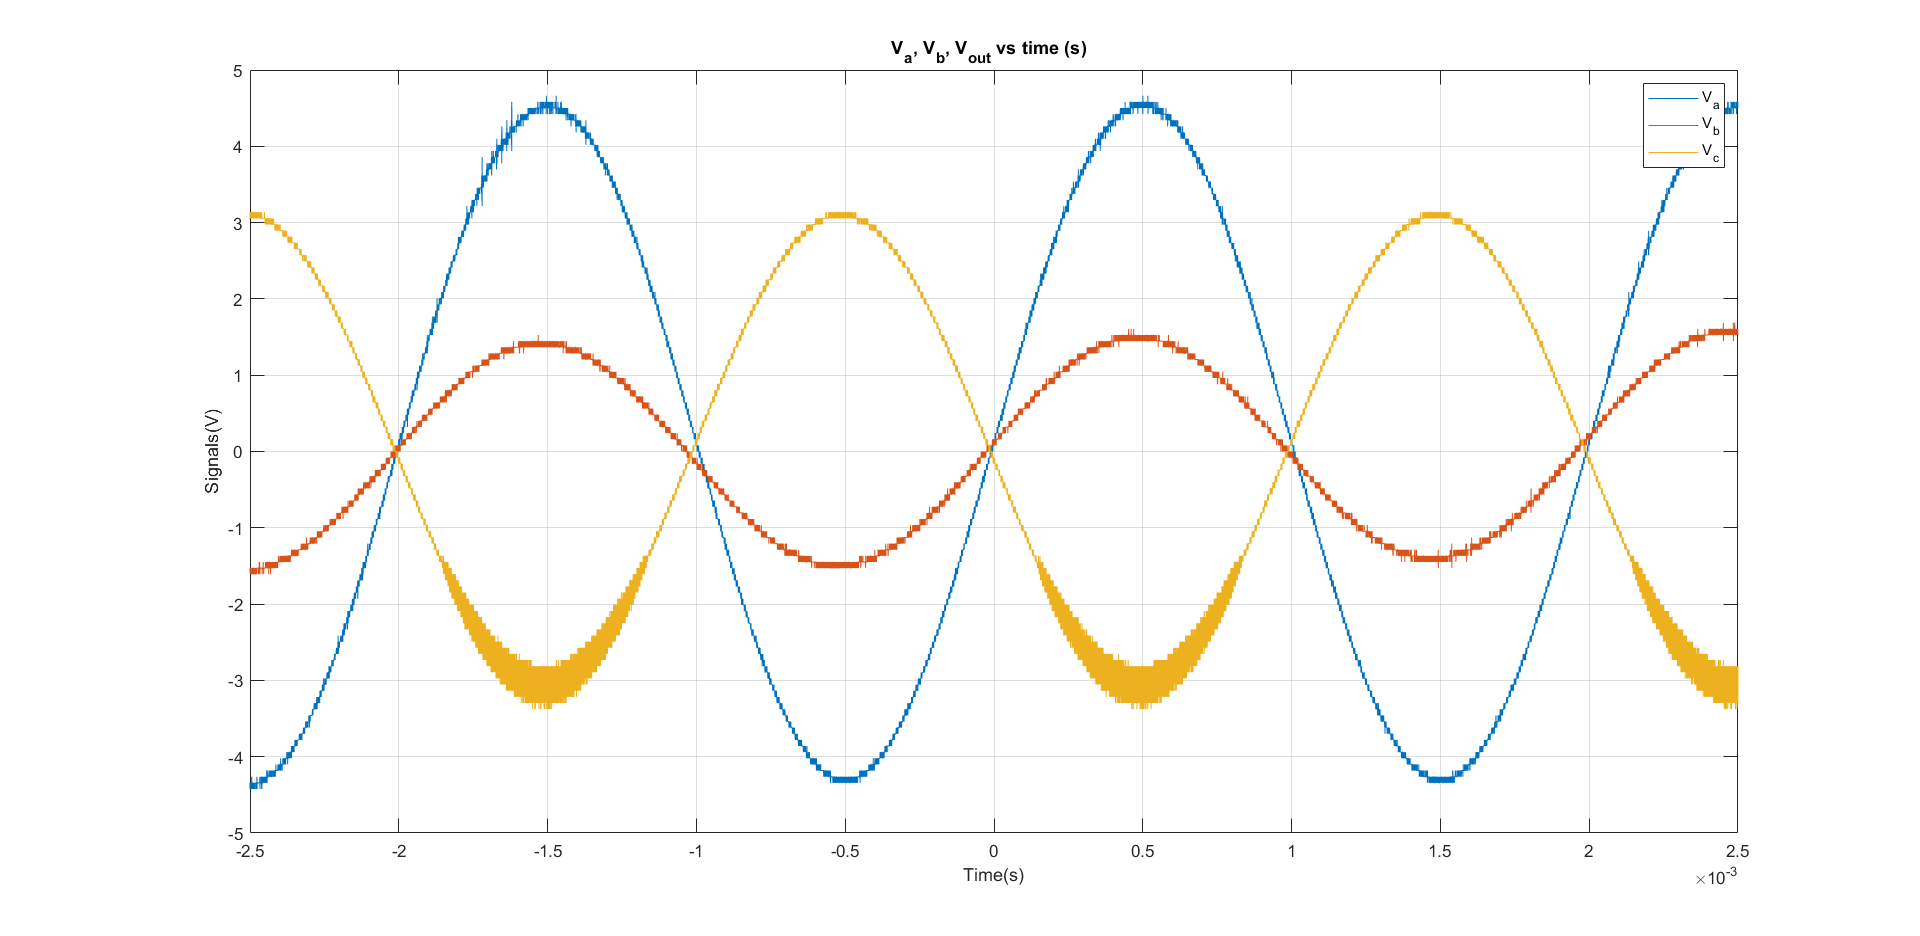
\includegraphics[width=0.6\textwidth]{5.png}
		\caption{Circuit schematic for the step 5}
	\end{figure} 

	\begin{figure}[htp] \centering{
		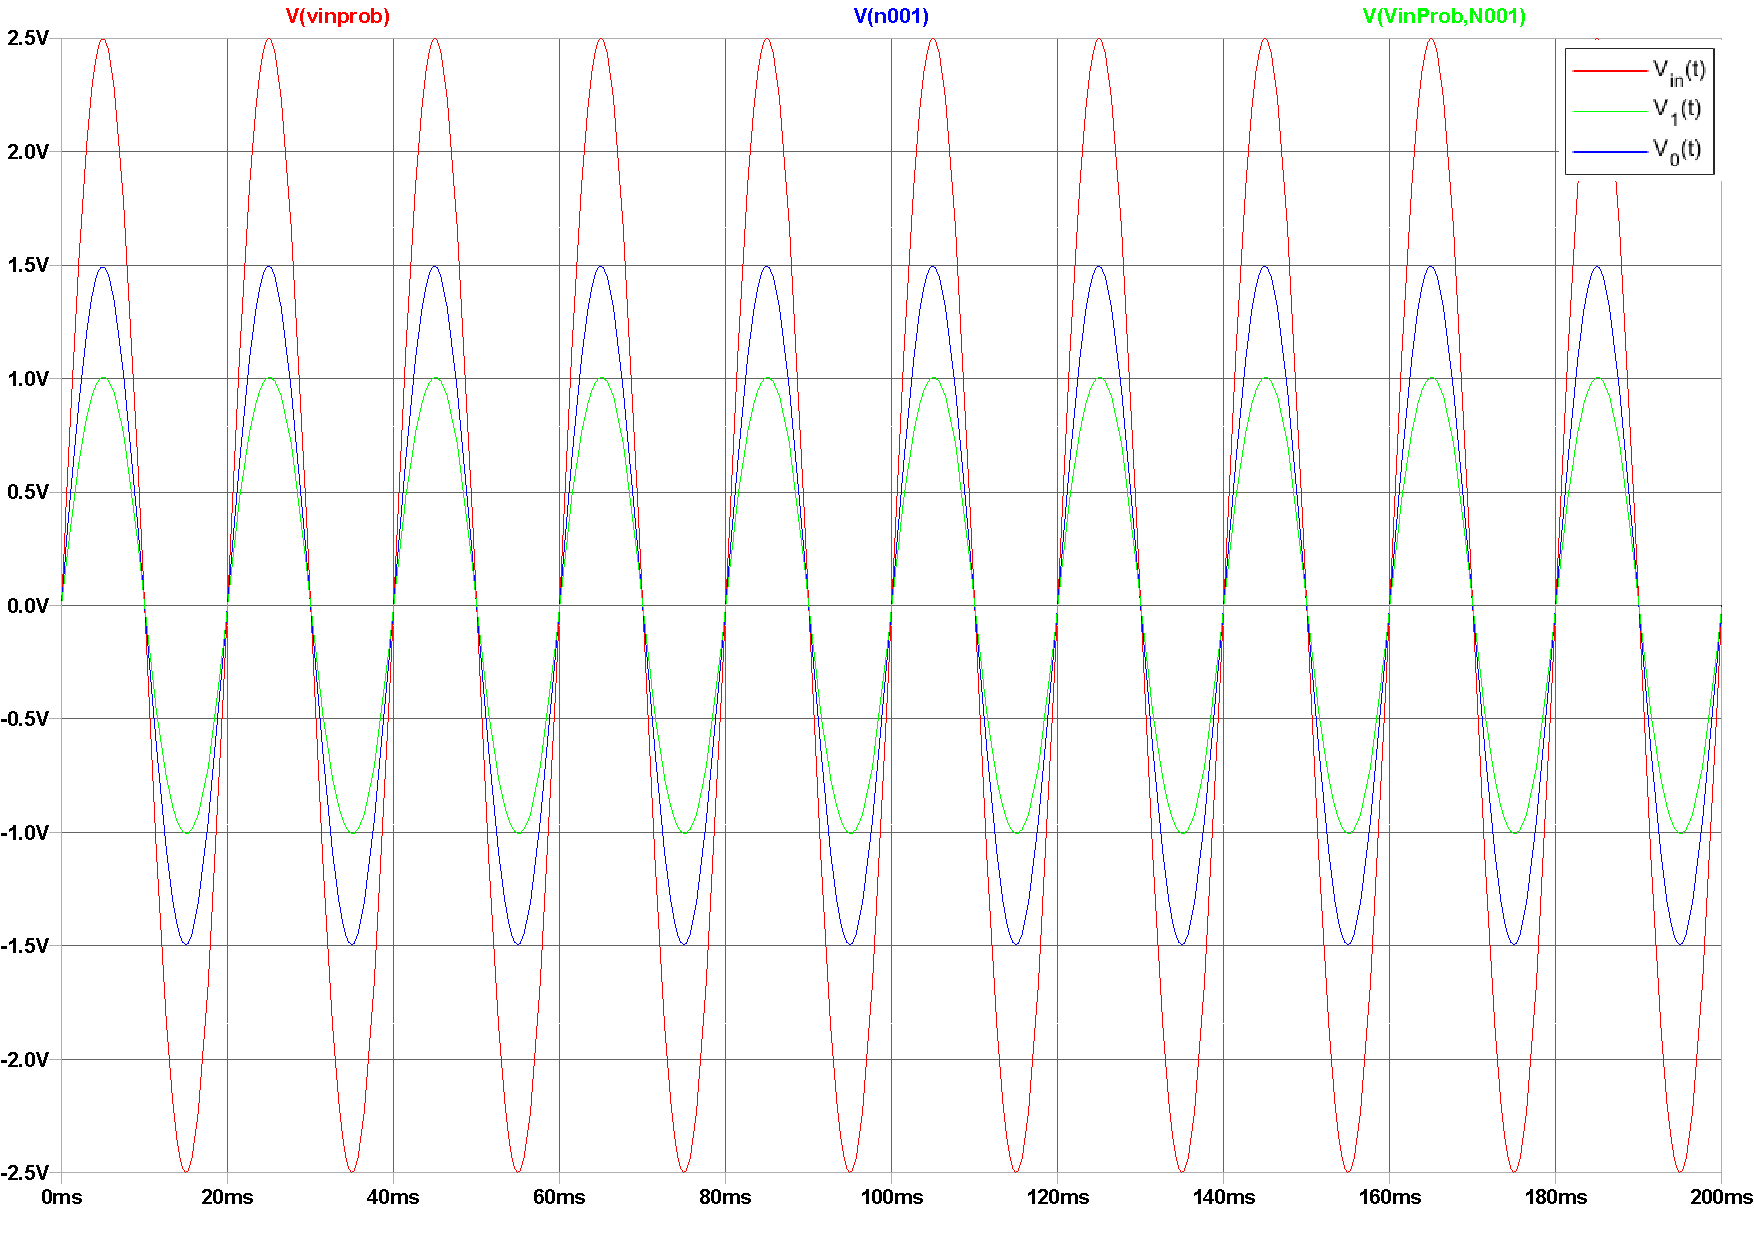
\includegraphics[scale=0.25]{2a_plot.pdf}}
		\caption{Experiment 2}
\end{figure}
	